\documentclass[10pt,a4paper]{article}
\usepackage[utf8]{inputenc}
\usepackage{amsmath}
\usepackage{amsfonts}
\usepackage{amssymb}
\usepackage{tikz}
\usepackage{graphicx}
\author{James Lee}
\title{5th Assignment of Computational Physics}
\begin{document}
	\maketitle
	\begin{abstract}
		In this report I present to you the numerical solution to Problem 1.6.
	\end{abstract}
	\section{Introduction}
	This program aims to calculate population growth problem.\\
	Population growth problem is a very complicated anthropological problem for it will be influenced by many factors. There are various mathematical models that are used to study population dynamics. In the following discussions, I will present to you two of these models.
	\subsection{Exponential population growth}
	Exponential growth describes unregulated reproduction. It is very unusual to see this in nature. In the last 100 years, human population growth has appeared to be exponential. In the long run, however, it is not likely. Paul Ehrlich and Thomas Malthus believed that human population growth would lead to overpopulation and starvation due to scarcity of resources. They believed that human population would grow at rate in which they exceed the ability at which humans can find food. In the future, humans would be unable to feed large populations. The biological assumptions of exponential growth is that the per capita growth rate is constant. Growth is not limited by resource scarcity or predation.\\
	ODE to describe this model:
	\begin{equation}
	\frac{dN}{dt}=rN
	\end{equation}
	\subsection{Logistic population growth}
	Logistics comes from the French word logistique, which means to compute. Population regulation is a density-dependent process, meaning that population growth rates are regulated by the density of a population. Think of the analogy of a thermostat. When the temperature is too hot, the thermostat turns on the AC to decrease the temperature back to homeostasis. When the temperature is too cold, the thermostat turns on the heater to increase the temperature back to homeostasis. Likewise with density dependence. Whether the population density is high or low, population dynamics returns the population density to homeostasis.\\
	In our model, this problem is described by a simple ODE:
	\begin{equation}
	\frac{dN}{dt}=aN-bN^2
	\end{equation}    
    Let me illustrate the given terms in the ODE. The first term $aN$ corresponds to the birth of new members, while the second term $-bN^2$ corresponds to the deaths. Notice that the death term is proportional to $N^2$ as food will be harder to find when $N$ is large.\\
    We should notice that when $b=0$, the Logistic growth reduces to exponential growth. Thus, studying this ODE under different parameters also provides us knowledge of exponential growth.\\ 
    In the following discussion I will use Euler method to solve this ODE.
    
    \section{Main Content}
    \subsection{$a=1, b=0$ case}
    Imagine an earth where no one will have to worry the threat of Death! On that earth, we will be able to learn physics from Einstein himself. How tempting is that?\\
    However, mathematics will soon tear up this fantasy, as this earth has to be infinitely large to fill all these people.\\   
    The analytical solution to case is:
    \begin{equation}
    N=N(0)e^{at}
    \end{equation}
    The numerical solution to this case will be plotted below:
    \begin{figure}[htbp]
    	\centering
    	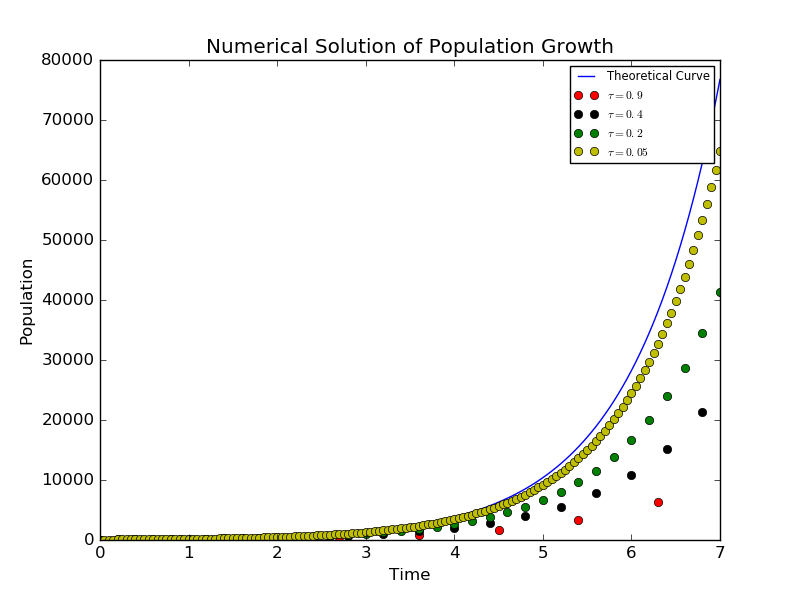
\includegraphics[width=5in]{Population.png}
    	\caption{Numerical Solutions with different $\tau$}
    \end{figure}
    Notice that solutions corresponding to this ODE is unrealistic, for the population will grow at a monstrous rate. On such an earth, wandering around will be regarded as a luxurious activity, for there are two many people blocking the ways!
    
   \subsection{Fixed $a$ with Varying $b$}
   Given the ODE, the only parameter that will influence the evolution is $a/b$. Thus, in order to study the evolution we should set $a$ fixed and let $b$ vary. This treatment can be interpreted as a family of evolution curves with different death rate.\\
   We set $a=1$ with $b$ varying.\\
   Analytically, there are three types of solutions corresponding to the ODE.\\
    1. Increasing population. (Relatively low death rate)\\
    2. Stable population. (Death rate neither high nor low)\\
    3. Decreasing population. (Relatively high death rate)\\
    These properties should be reflected in our numerical solution.\\ 
    The numerical solution to this case will be plotted in figure \ref{Figure_2}:
    \begin{figure}[htbp]
    	\centering
    	\includegraphics[width=5in]{Population_2.png}
    	\caption{Numerical Solutions with different $b$\label{Figure_2}}
    \end{figure}
    As we can see in this figure, three types of solutions are presented. Notice that when $b=0.5$, the system behaves much like an exponential growth. This is reasonable due to  correspondence principle. However, if we zoom out a little bit, we will immediately find that $b=0.5$ curve cannot grow forever.\\
    There is one other thing I would like to mention. When first applying Euler method for these relatively low $a/b$ ratio, I chose $N(0)=50$ only to find the solution blown up. Further investigation showed that this is caused by the limited precision of variables. This incident assured me to check the precision of the numerical value of the variables more carefully.
    
    \section*{Acknowledgement}
    When tackling this assignment, I benefitted a lot from the valuable discussions with Liu Xingchen. I would like to thank him for pointing out several grammar errors I made, also, for his willingness to discuss with me.
    
    \begin{thebibliography}{99}
    	\bibitem{}Hunter J, the Matplotlib Documentation, 2016
    	\bibitem{}Giordano N.J, Nakanishi H, Computational Physics, Pearson Education, 2007
    \end{thebibliography} 
\end{document}